% \subsection{Experimental Setting}
In this section, we conduct several experiments on two data sets: (1) the productional e-commerce data set; (2) the publicly available music data set.  We compare our proposed method HBayes against several other \emph{state-of-the-art} recommendation methods which are briefly described as follows:
%\textbf{KNN} \cite{koren2010factor}:

\textbf{HSR} \cite{wang2015exploring}: is an item-based recommendation approach that employs a special non-negative matrix factorization for exploring the implicit hierarchical structure of users and items so the user preference towards certain products are better understood.  We adopt HSR  as one baseline. 

\textbf{HPF} \cite{gopalan2015scalable}: generates a hierarchical Poisson factorization model for better modeling users' rating towards certain items based upon each one's latent preferences.  Unlike proposed HBayes, HPF does not leverage the content item feature for constructing the hierarchical structure. We adopt HPF as another baseline.

\textbf{SVD++} \cite{mnih2008probabilistic, koren2008factorization}: combines the collaborative filtering approach and latent factor approach, so to provide a more accurate neighboring based recommendation result.  We adopt SVD++ as another baseline.

\textbf{CoClustering} \cite{george2005scalable}: another collaborative filtering flavored recommendation approach based on weighted co-clustering improvements that simultaneously cluster users and items.  We adopt CoClustering as another baseline.

\textbf{Fatorization Machine (FM)} \cite{rendle2010factorization}: combines support vector machines (SVM) with factorization models which takes the advantage of SVM meanwhile overcomes the feature sparsity issues.  In this paper, we adopt LibFM implementation mentioned in \cite{rendle2012factorization} as another baseline.

\textbf{LambdaMART} \cite{burges2010ranknet}: is the boosted tree version of LambdaRank \cite{donmez2009local}, which is based on RankNet \cite{burges2005learning}.  LambdaMART proves to be a very successful approach for ranking as well as recommendation.  We include LambdaMART as another baseline. 

\subsection{Evaluation Metrics}
Throughout the experiment section, we compare HBayes against other baselines on the testing held-out data set under the 5-fold cross-validation setting.  For each fold, after fitting the model on the training set, we form the predictive rating for the test set, and generate the top $M$ samples from each method for recommendation.  Regarding with metrics, we adopt precision and recall as well as F1-score for measuring the product retrieval quality and normalized discounted information gain (NDCG) for measuring the recommendation's ranking quality.  More specifically, precision, recall, and F1-score are defined as follows:

\begin{eqnarray}
\text{precision}_M & = & \frac{\text{\# of products clicked in top }M}{M} \nonumber \\
\text{recall}_M & = & \frac{\text{\# of products clicked in top }M}{\text{\# of products the user clicked}} \nonumber\\
\text{F1-score@} M & = & 2\frac{\text{precision}_M\cdot \text{recall}_M}{\text{precision}_M + \text{recall}_M} \nonumber
\end{eqnarray}

discounted cumulative gain (DCG) measures the ranking quality based on the result list product positions, defined as:
\begin{eqnarray}
\text{DCG}_M & = & \sum_{i=1}^M\frac{r_i}{\log_2(i+1)} =  r_1 + \sum_{i=2}^M\frac{r_i}{\log_2(i+1)}\nonumber
\end{eqnarray}
sorting all potential products to produce the maximum possible DCG through position $M$, also called Ideal DCG (IDCG).  For each user, we can define NDCG as follows:
\begin{eqnarray}
\text{NDCG}_M & = & \frac{\text{DCG}_M}{\text{IDCG}_M}\nonumber
\end{eqnarray}

\subsection{Recommendation on E-commerce Data}
The first data set is collected from a large e-commerce company.  In this dataset, each sample represents a particular product which is recorded by various features including: category, title, and other properties, etc.  Meanwhile, the users' click and purchase history are also recorded. Throughout the experiment, positive labels indicate that certain products in recommendation are clicked by the user, whereas negative samples indicate that products in recommendation are skipped by the user.  By data cleaning and preprocessing for merging duplicated histories, removing users with too few historical samples, the final data set ends up of $895$ users, $81,223$ products, $5,535$ brands with $380,595$ uniquely observed user-item pairs.  In average, each user has $425$ products records, ranging from $105$ to $2,048$, and $61.2\%$ of the users have fewer than $425$ product clicking records.  For each product, we encode each popularity and category features to a separate $20$ dimension vector; title and product property feature to a separate $50$ dimension vector.   The total dimension for each product sample ends up of $140$.

\subsubsection{Feature Analysis}
The e-commerce data are composed by four types of features: (1) product popularity; (2) product category; (3) product title; (4) product properties and we briefly explain their physical meanings and how we preprocess the data as follows:

\textbf{Product Popularity (POP):} product popularity is a measure of the prevalence of a product in the dataset. In general, consumers have a preference for a particular product during a period of time. This phenomenon is pretty common in apparel product. For a particular product $i$, the popularity is computed as follows: $\mathrm{\scriptsize POP}_{i} \coloneqq \frac{n_{x_i}}{\mathcal{N}_\mathbf{x}}$, where $n_{x_i}$ are the number of orders or the contribution of gross merchandise volume (GMV) for product $i$,  and $\mathcal{N}_\mathbf{x} = \sum_{\forall x_i}n_{x_i}$ is the summation of $n_{x_i}$ for all such products in the dataset.

\textbf{Product Category (CID):}  user actions towards a single item such as click, purchase, etc. are typically sparse event, while more patterns could be recognized if we cluster different items into different groups based on their functionalities and utilities.  In most e-commerce websites, such a categorical hierarchy exists.    We encode each product's category into a high dimensional vector via one-hot encoding and adjust the feature weights by the popularity of such category.

\textbf{Product Title (TITLE):} product titles are created by vendors and they are typically in the forms of natural languages indicating the product functionality and utility.  Examples could be like 'INMAN short sleeve round neck triple color block stripe T-shirt 2017'.  We preprocess the product titles by generating the sentence vector embedding based on \cite{de2016representation}.  The main idea is to average the word weights in the title sentence based on the inverse document frequency (IDF) value of each individual word involved.

\textbf{Product Property Features (PROP):} other product metadata features are also provided in this dataset. For example,  product 'color' feature takes value of "black", "white", "red", etc, and product 'size' feature takes value of "S", "M", "L", "XL", etc.  Similar as category features, each product property is first encoded as a binary vector $\bm{x}_i \in \{0, 1\}^{|N|}$, where $N$ denotes the set of all possible corresponding product values.  Then we encode all property binary vectors into a fixed length ($50$ throughout the experiment) vector. %We can see the property features vector is generally sparse since each product is only associated with a small number of feature.  % how did we do the encoding??

On one hand by utilizing more types of product features HBayes in general reaches better results in terms of precision-recall metrics.  We report PR-AUC in table (\ref{tab:features_cmp}) to prove our argument.   On the other hand, more features typically needs much more training time.  Figure (\ref{fig:train_time_cmp}) reports the change in likelihood comparing against training time (minutes) for each feature combination case \footnote{The experiment is conducted via the same linux qual core 2.8 GHz Intel Core i7 macbook with 16 Giggabytes of memory}.   It is shown that by taking one POP feature set, model takes less than 5 minutes to converge while taking feature combination POP+CID+TITLE+PROP leaves us more than 6 hours in training.   

\begin{table}[htb]
\centering
\begin{tabular}{l|c}
\toprule
\textbf{Features} & \textbf{PR AUC} \\
\hline
POP & 0.0406 \\
\rowcolor{mygray}
POP+CID & 0.0414 \\
POP+CID+TITLE & 0.0489 \\
\rowcolor{mygray}
POP+CID+TITLE+PROP & 0.0491 \\
\bottomrule
\end{tabular}
\caption{Model performance under different feature combinations in terms of PR AUC}
\label{tab:features_cmp}
\end{table}



\begin{figure*}[!htb]
\minipage{0.32\textwidth}
  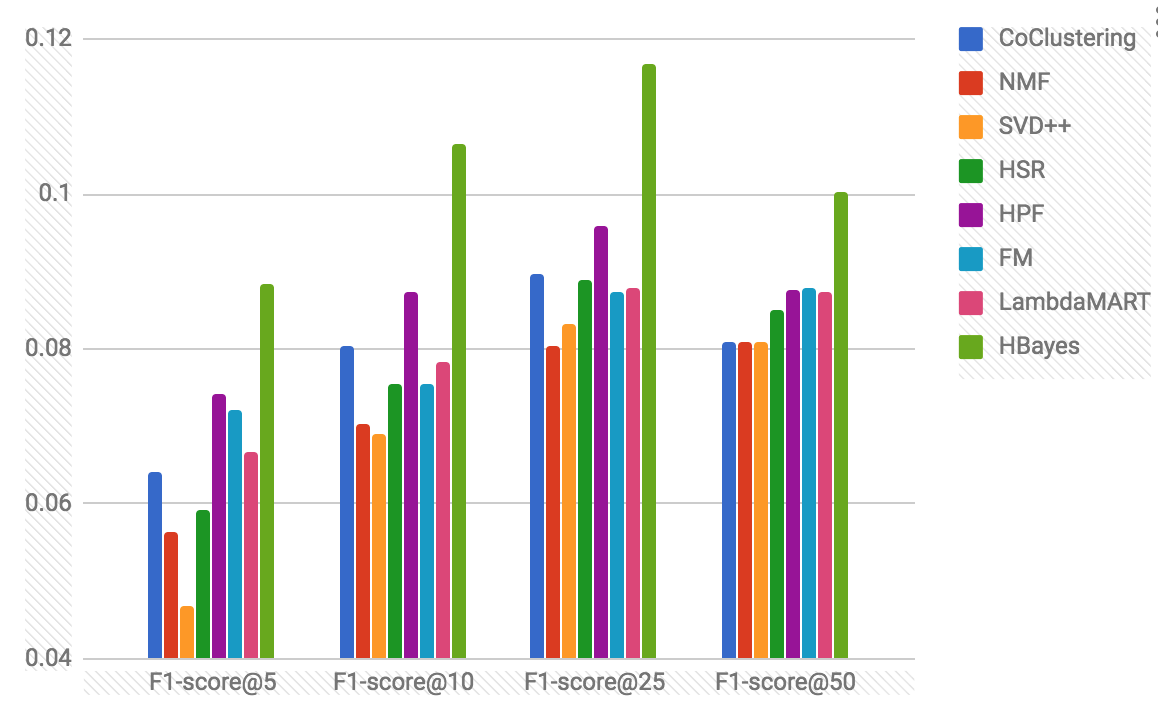
\includegraphics[width=\linewidth]{fig/test}
  \caption{F1@K on \emph{Apparel} data.}\label{fig:awesome_image1}
\endminipage\hfill
\minipage{0.32\textwidth}
  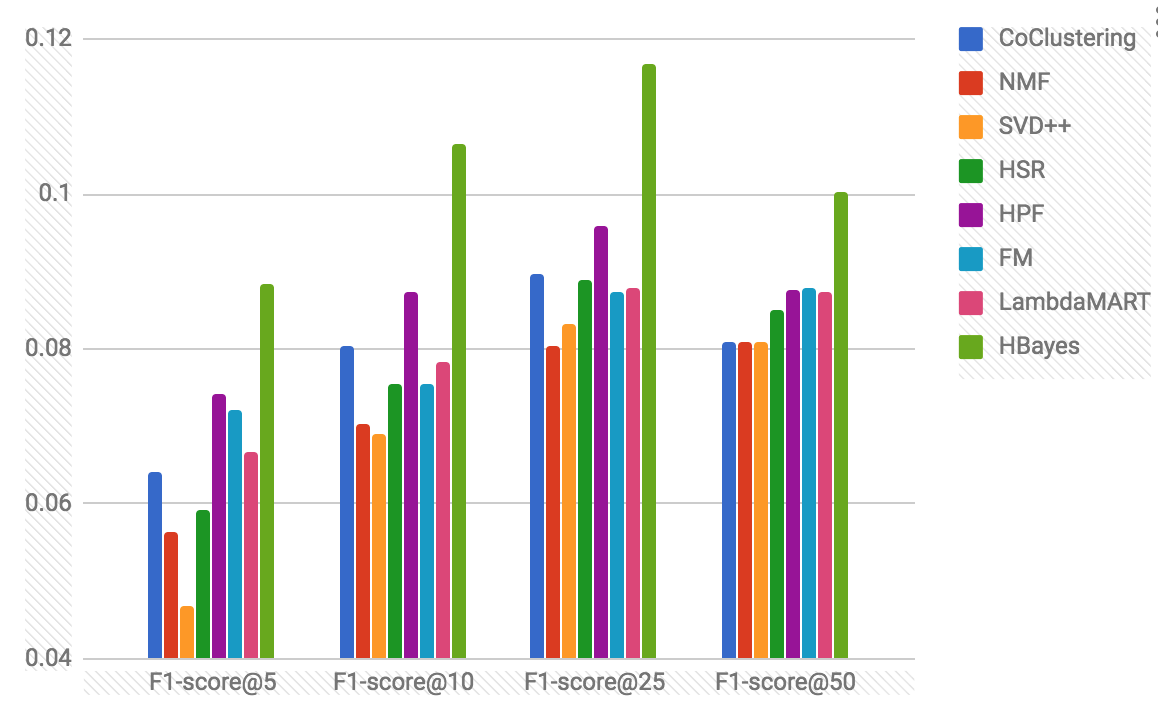
\includegraphics[width=\linewidth]{fig/test}
  \caption{Precision@K on \emph{Apparel} data.}\label{fig:awesome_image2}
\endminipage\hfill
\minipage{0.32\textwidth}%
  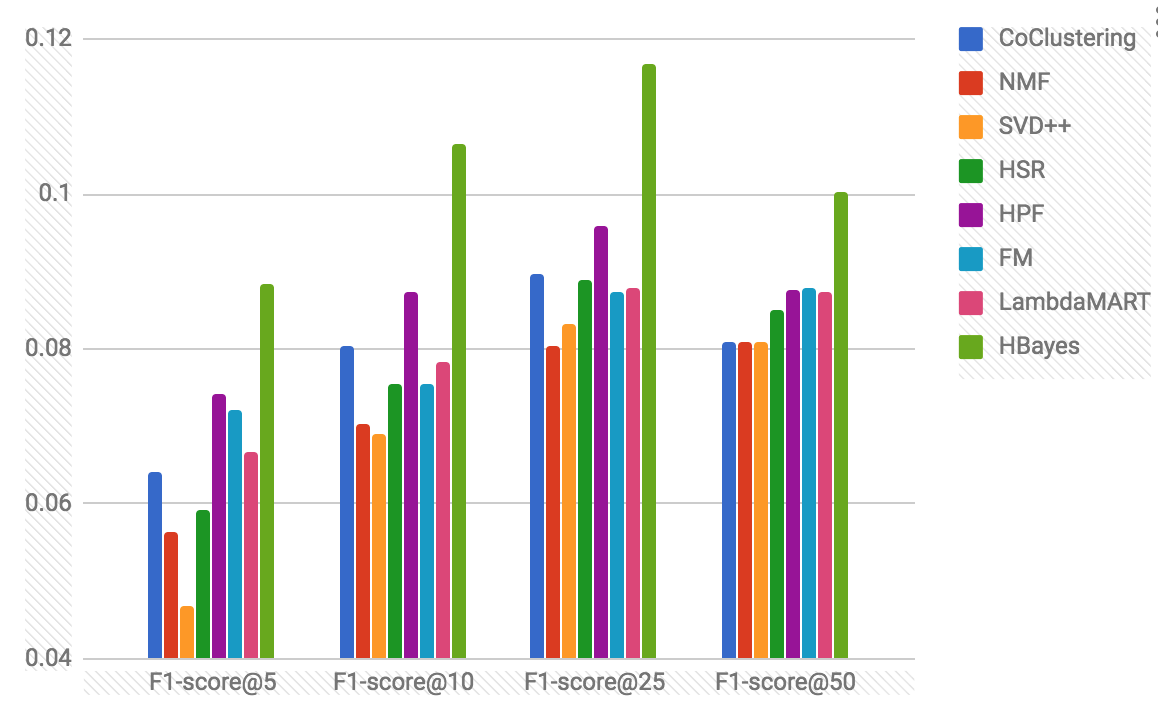
\includegraphics[width=\linewidth]{fig/test}
  \caption{Recall@K on \emph{Apparel} data.}\label{fig:awesome_image3}
\endminipage
\end{figure*}


\begin{figure*}[!htb]
\minipage{0.32\textwidth}
  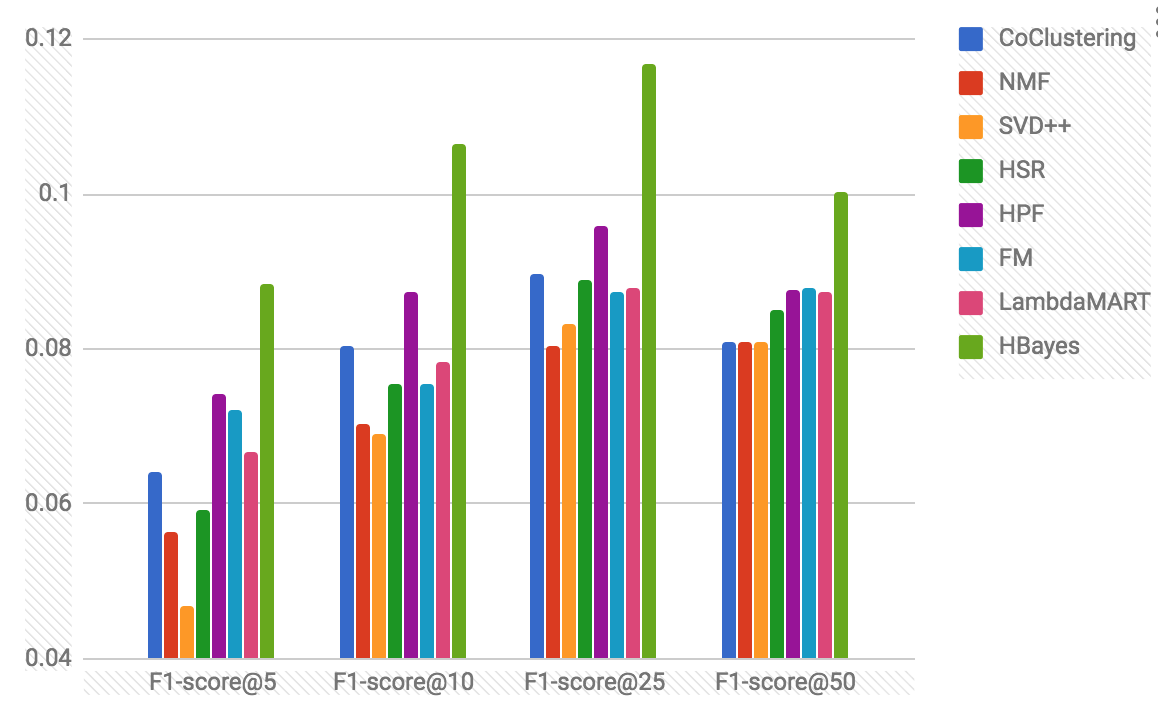
\includegraphics[width=\linewidth]{fig/test}
  \caption{F1@K on \emph{Music} data.}\label{fig:awesome_image1}
\endminipage\hfill
\minipage{0.32\textwidth}
  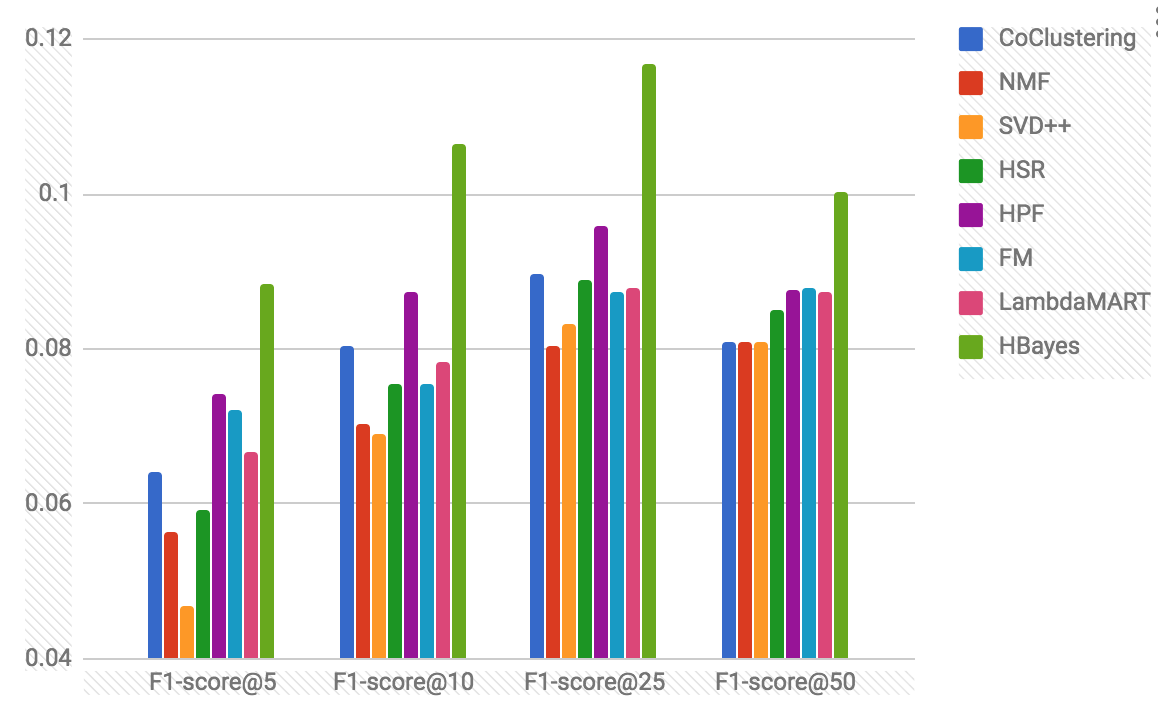
\includegraphics[width=\linewidth]{fig/test}
  \caption{Precision@K on \emph{Music} data.}\label{fig:awesome_image2}
\endminipage\hfill
\minipage{0.32\textwidth}%
  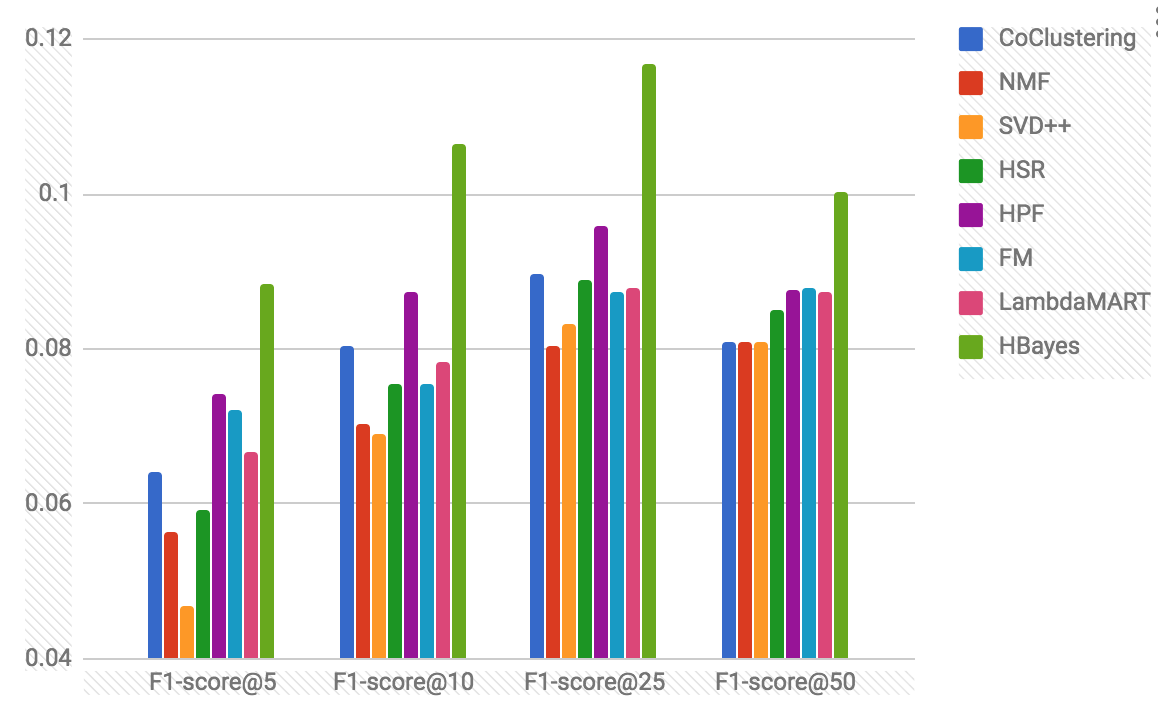
\includegraphics[width=\linewidth]{fig/test}
  \caption{Recall@K on \emph{Music} data.}\label{fig:awesome_image3}
\endminipage
\end{figure*}

\begin{figure}[htb]
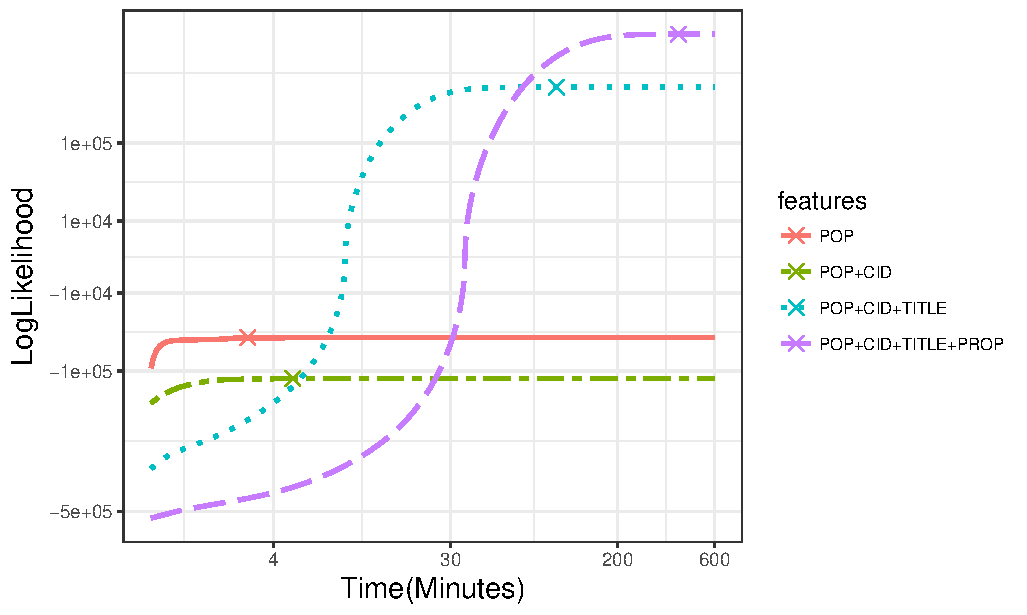
\includegraphics[width=0.9\columnwidth,height=0.5\columnwidth]{fig/Lik_time}
\caption{Training time under different feature combinations on e-commerce recommendations}
\label{fig:train_time_cmp}
\end{figure}

% \begin{figure}[htb]
% 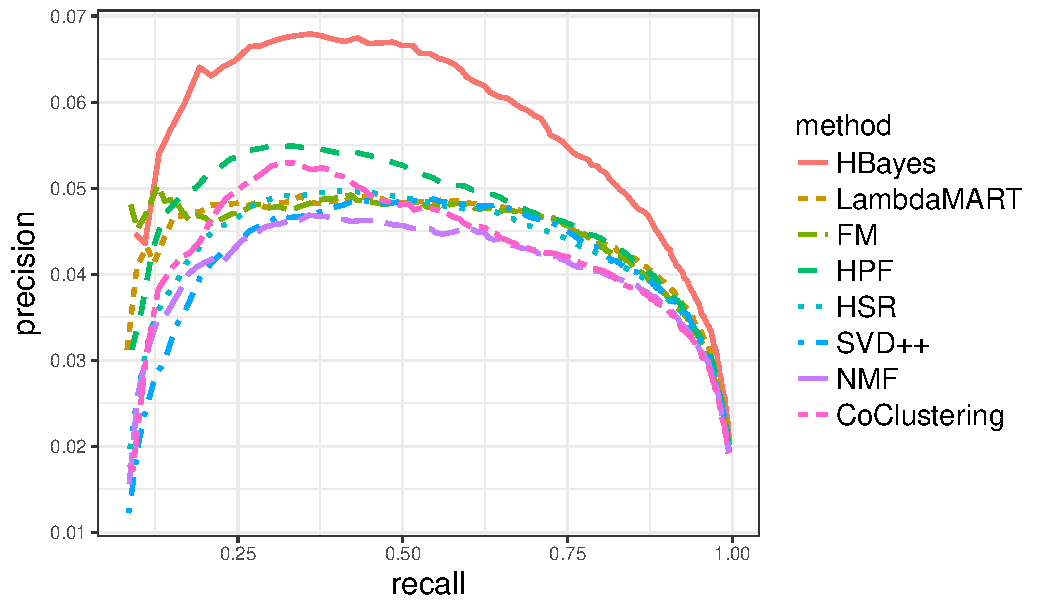
\includegraphics[width=0.9\columnwidth,height=0.5\columnwidth]{fig/pre-recall}
% \caption{PR curves on e-commerce recommendations}
% \label{fig:perf_cmp}
% \end{figure}

% \begin{table}[htb]
% \begin{center}
% \scalebox{0.7}{
% \begin{tabular}{l|cccc}
% \toprule
% \textbf{Method} & \textbf{F1-score@5} & \textbf{F1-score@10} & \textbf{F1-score@25} & \textbf{F1-score@50} \\
% \hline
% \rowcolor{mygray}
% CoClustering & 0.0640 & 0.0804 & 0.0896 & 0.0809 \\
% NMF & 0.0565 & 0.0702 & 0.0832 & 0.0809 \\
% \rowcolor{mygray}
% SVD++ & 0.0467 & 0.0689 & 0.0875 & 0.0865\\
% HSR & 0.0592 & 0.0755 & 0.0889 & 0.0850\\
% \rowcolor{mygray}
% HPF & 0.0741 & 0.0874 & 0.0960 & 0.0876\\
% FM & 0.0720 & 0.0756 & 0.0874 & 0.0880\\
% \rowcolor{mygray}
% LambdaMART & 0.0667 & 0.0782 & 0.0879 & 0.0874\\
% HBayes & \textbf{0.0885} & \textbf{0.1065} & \textbf{0.1168} & \textbf{0.1002}\\
% \bottomrule
% \end{tabular}}
% \end{center}
% \caption{F1-score on e-commerce recommendations}
% \label{F!-score_cmp}
% \end{table}

\begin{table}[htb]
\begin{center}
\scalebox{0.7}{
\begin{tabular}{l|cccc}
\toprule
\textbf{Method} & \textbf{NDCG@5} & \textbf{NDCG@10} & \textbf{NDCG@25} & \textbf{NDCG@50} \\
\hline
\rowcolor{mygray}
CoClustering & 0.1288 & 0.1637 & 0.2365 & 0.3050 \\
NMF & 0.1249 & 0.0156 & 0.2272 & 0.3020 \\
\rowcolor{mygray}
SVD++ & 0.1138 & 0.1487 & 0.2287 & 0.3073\\
HSR & 0.1266 & 0.1603 & 0.2354 & 0.3107 \\
\rowcolor{mygray}
HPF & 0.1412 & 0.1757 & 0.2503 & 0.3229 \\
FM & 0.1363 & 0.1592 & 0.2291 & 0.3117\\
\rowcolor{mygray}
LambdaMART & 0.1287 & 0.1585 & 0.2304 & 0.3123\\
HBayes & \textbf{0.1557} & \textbf{0.1974} & \textbf{0.2871} & \textbf{0.3590}\\
\bottomrule
\end{tabular}}
\end{center}
\caption{NDCG on e-commerce recommendations}
\label{NDCG_cmp}
\end{table}

\subsubsection{Performance Comparison}
We first report the model performance regarding precision-recall for HBayes and other baselines in Figure (\ref{fig:perf_cmp}).  As shown when each method recommend fewer number of products, HBayes, FM, shares similar performance, with the increment of recommended items, HBayes becomes more efficient, in the sense of picking more number of products that users take interest in.  In terms of overall PR-AUC, HBayes is able to reach $0.053$, while beating the second best LambdaMART of $0.041$ PR-AUC by $29.3\%$ percent.   In terms of F1-score, we are the best cross out different number of products recommended by beating against the second best LambdaMART by $29\%$ in average.  

Regarding with ranking quality, HBayes is also superior against other baselines through out different items recommended.  Specially HBayes beats the second best CoClustering at $M=5,10,25$ by $21.0\%$ in average and LambdaMART at $M=50$ by $15.0\%$.  

\subsubsection{Model Learning Analysis}
\begin{figure}
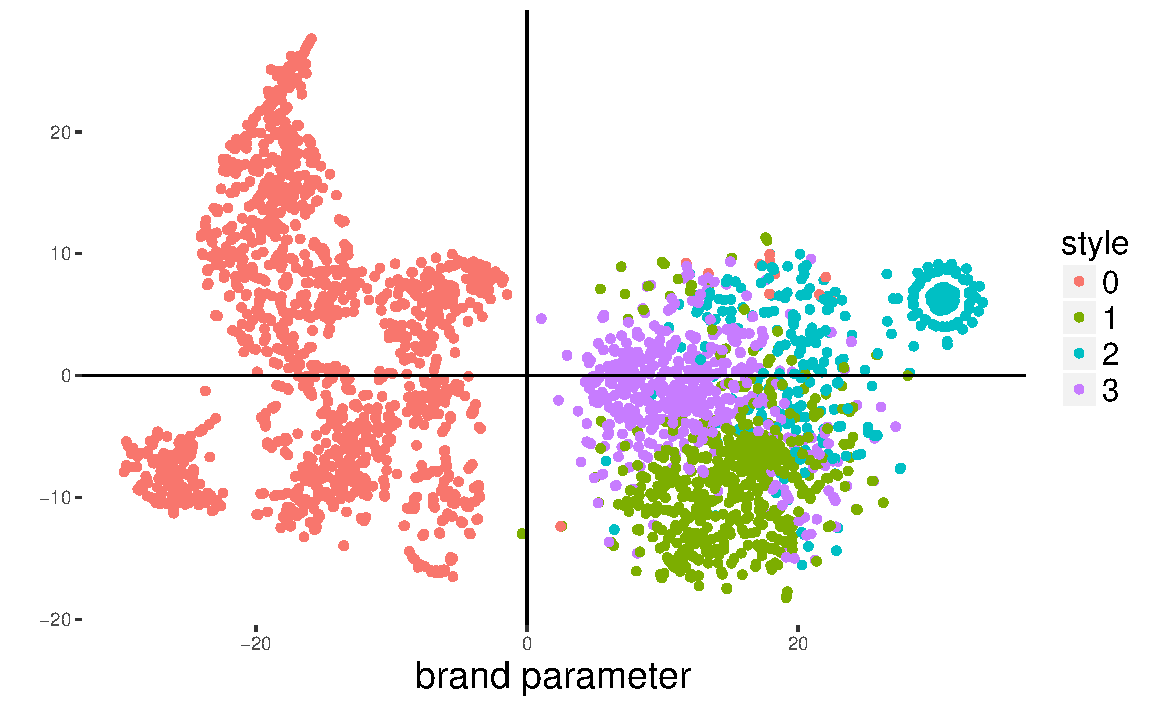
\includegraphics[width=0.58\columnwidth,height=3cm]{fig/brand_tsne}
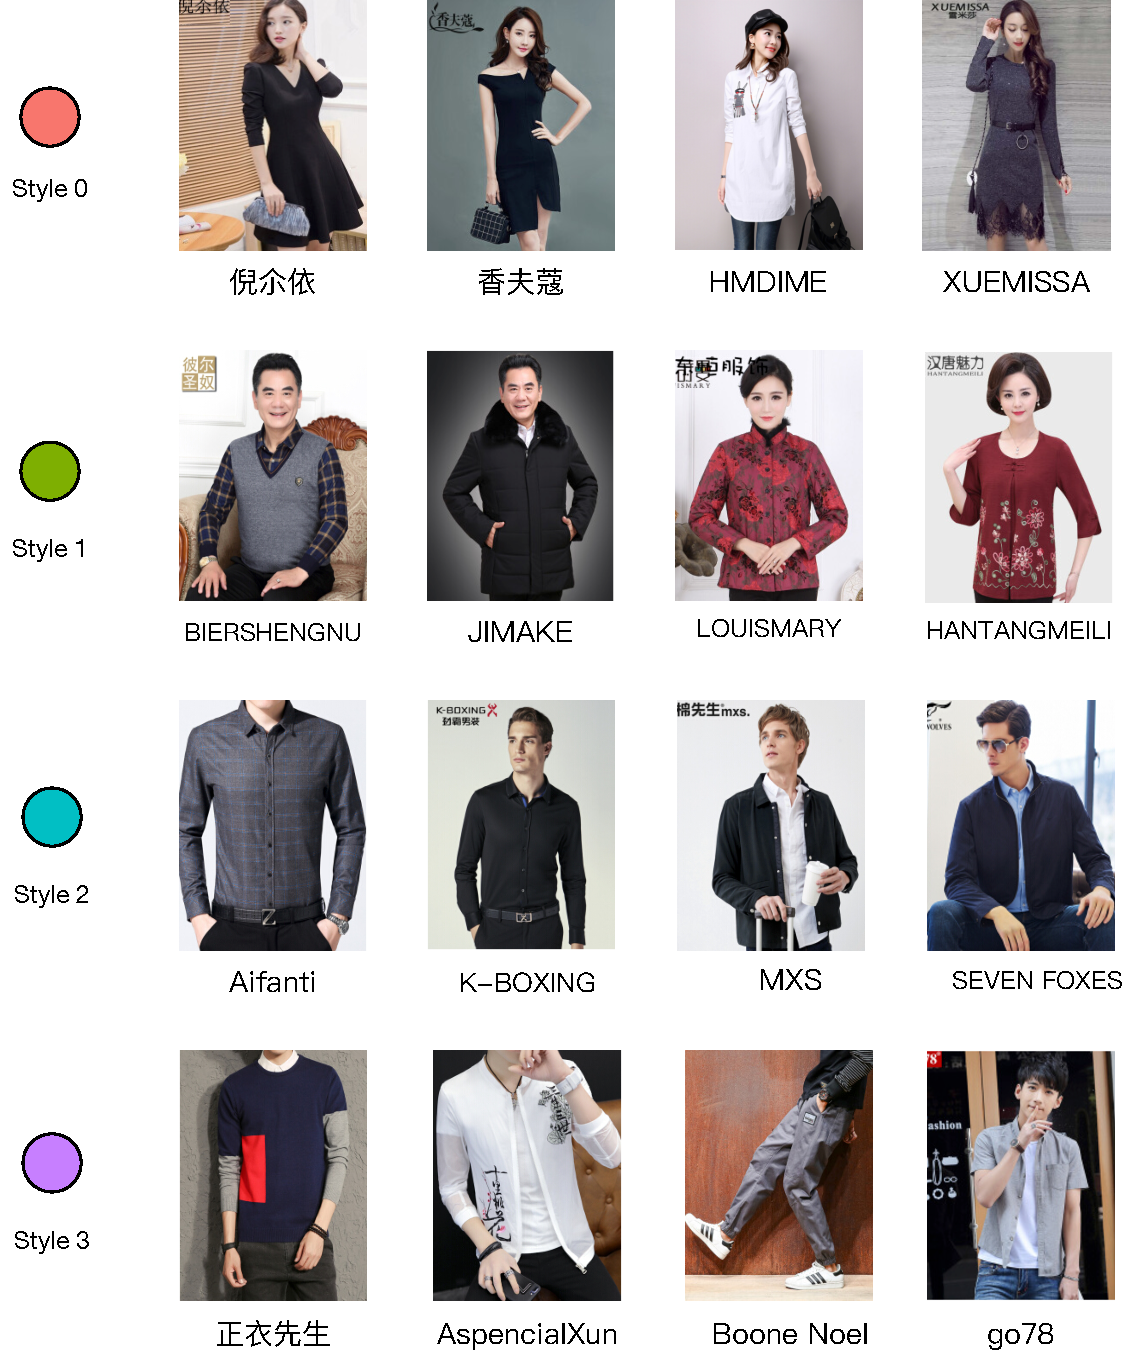
\includegraphics[width=0.39\columnwidth,height=4cm]{fig/style-brand}
\caption{tSNE of four latent apparel style clusters}
\label{fig:tsne-represntation-style-cluster}
\end{figure}

Like mentioned in Sec.\ref{sec:method}, HBayes learns the latent style clusters, and group different brands of products based on their different hidden style representations.  Figure (\ref{fig:tsne-represntation-style-cluster}) shows the tSNE\cite{maaten2008visualizing} representation of different style clusters learned by HBayes and we randomly pick four samples within each clusters and present their product images at the right subfigure.  As shown, cluster one which takes a great proportion of apparel products are seemingly about young stylish female garment.  This is making sense since a majority of apparel customers are young females while most products are focusing on this group of customer audience.    The second cluster seems about senior customers who are in elder age.   Interestingly, the third cluster and the fourth cluster which are closed tied together are both about young male customers.  However, the third cluster seems more focusing on office business men style garment while the fourth cluster is more focusing on asian street styles.  This indicates us that our hierarchical Bayesian model does learn meaningful intrinsic garment styles from apperal products with customer behavioral data.   

\subsection{Recommendation on Last.fm Music Data}
The second data set is collected from Last.fm dataset \cite{Celma:Springer2010} and Free Music Archive (FMA) \cite{FMA}. Last.fm is a publicly available dataset contains the whole listening habits (till May, 5th 2009) for $1,000$ users. FMA is an open and easily accessible dataset providing $917$ GiB and $343$ days of Creative Commons-licensed audio from $106,574$ tracks, $16,341$ artists and $14,854$ albums, arranged in a hierarchical taxonomy of $161$ genres. It also provides full-length and high quality audios with precomputed features.  In our experiment, tracks in Last.fm dataset were further intersected with FMA dataset for better feature generation.  The resulting dataset contains $500$ users, $16,328$ tracks and $36$ genres.

\subsubsection{Performance Comparison}
We conduct the same set of experiments as we do for e-commerce data and report different precision-recall performances in Figure (\ref{fig:perf_cmp_music}).  


% \begin{figure}[htb]
% 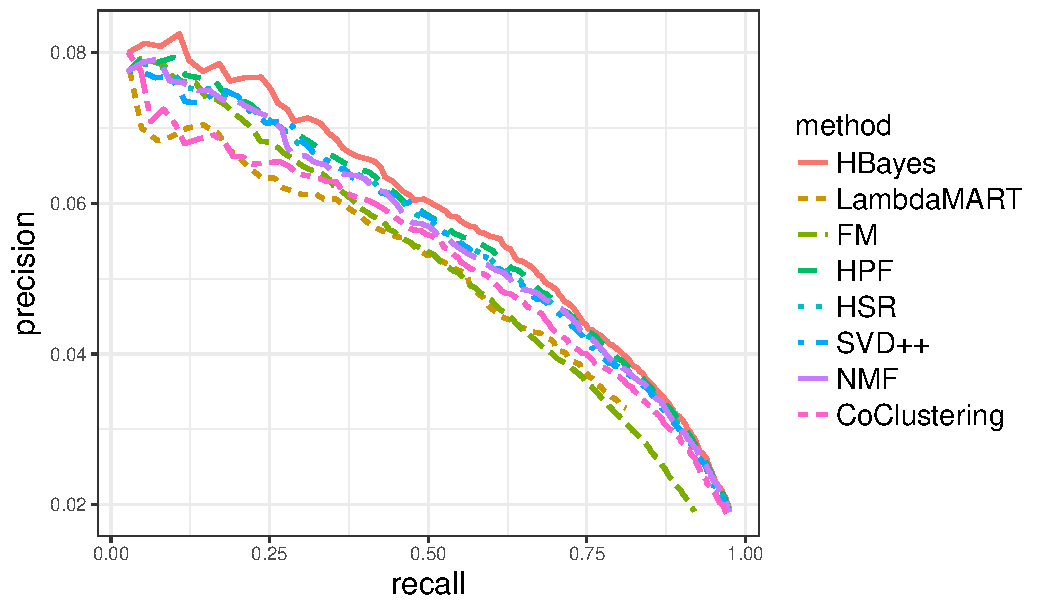
\includegraphics[width=0.9\columnwidth,height=0.5\columnwidth]{fig/Pre-recall_music}
% \caption{PR curves on Last.fm recommendations}
% \label{fig:perf_cmp_music}
% \end{figure}

% \begin{table}[htb]
% \label{F1-score_cmp_music}
% \begin{center}
% \scalebox{0.7}{
% \begin{tabular}{l|cccc}
% \toprule
% \textbf{Method} & \textbf{F1-score@5} & \textbf{F1-score@10} & \textbf{F1-score@25} & \textbf{F1-score@50} \\
% \hline
% \rowcolor{mygray}
% CoClustering & 0.0831 & 0.0986 & 0.1049 & 0.0915 \\
% NMF & 0.0913 & 0.1088 & 0.1075 & 0.0941 \\
% \rowcolor{mygray}
% SVD++ & 0.0903 & 0.1084 & 0.1084 & 0.0946\\
% HSR & 0.0916 & 0.1089 & 0.1083 & 0.949\\
% \rowcolor{mygray}
% FPF & 0.0931 & 0.1097 & 0.1092 & 0.961\\
% FM & 0.0863 & 0.1041 & 0.1059 & 0.942\\
% \rowcolor{mygray}
% LambdaMART & 0.0622 & 0.0788 & 0.0995 & 0.0987\\
% HBayes & \textbf{0.0962} & \textbf{0.1159} & \textbf{0.1107} & \textbf{0.0985} \\
% \bottomrule
% \end{tabular}}
% \caption{F1-score on Last.fm recommendations}
% \end{center}
% \end{table}

\begin{table}[htb]
\label{NDCG_cmp_music}
\begin{center}
\scalebox{0.7}{
\begin{tabular}{l|cccc}
\toprule
\textbf{Method} & \textbf{NDCG@5} & \textbf{NDCG@10} & \textbf{NDCG@25} & \textbf{NDCG@50} \\
\hline
\rowcolor{mygray}
CoClustering & 0.2415 & 0.2314 & 0.2289 & 0.2349 \\
NMF & 0.2556 & 0.2494 & 0.2368 & 0.2431 \\
\rowcolor{mygray}
SVD++ & 0.2493 & 0.2478 & 0.2381 & 0.2439\\
HSR & 0.2544 & 0.2495 & 0.2384 & 0.2448\\
\rowcolor{mygray}
HPF & 0.2584 & 0.2513 & 0.2405 & 0.2474\\
FM & 0.2527 & 0.2453 & 0.2284 & 0.2333\\
\rowcolor{mygray}
LambdaMART & 0.2372 & 0.2337 & 0.2272 & 0.2218\\
HBayes & \textbf{0.2655} & \textbf{0.2620} & \textbf{0.2455} & \textbf{0.2537}\\
\bottomrule
\end{tabular}}
\caption{NDCG on Last.fm recommendations}
\end{center}
\end{table}

For PR-AUC, HBayes (0.055) again beats against the second best, which is LambdaMART (0.043) by $27.9\%$.  In terms of F1-score, HBayes in average beats against LambdaMART by $14.0\%$.  Regarding with the ranking quality, HBayes beats against the second best, which is NMF  for $M=5,10,25$ by $4.20\%$ in average and SVD++ for $M=50$ by $4.02\%$.  









